\chapter{Active Directory}
\section{Terminology}

\subsection{NTDS.DIT}
\index{Active Directory!NTDS}
\label{win:NTDS}

The NTDS.DIT file can be considered the heart of Active Directory. It is stored
on a Domain Controller at \verb+C:\Windows\NTDS\+ and is a database that stores AD data such as information about user and group objects, group membership, and, most important to attackers and penetration testers, the password hashes for all users in the domain. Once full domain compromise is reached, an attacker can retrieve this file, extract the hashes, and either use them to perform a pass-the-hash attack or crack them offline using a tool such as Hashcat to access additional resources in the domain. If the setting Store password with reversible encryption is enabled, then the NTDS.DIT will also store the cleartext passwords for all users created or who changed their password after this policy was set. While rare, some organizations may enable this setting if they use applications or protocols that need to use a user's existing password (and not Kerberos) for authentication.


\section{AD objects}

\textbf{Users}
\index{Active Directory!user}

Users are considered leaf objects,  which means that they cannot contain any other objects within them.  Another example of a leaf object is a mailbox in Microsoft Exchange. A  user object is considered a security principal and has a security  identifier (SID) and a global unique identifier (GUID). User objects  have many possible attributes,  such as their display name, last login time, date of last password  change, email address, account description, manager, address, and more.  Depending on how a particular Active Directory environment is set up,  there can be over 800 possible user attributes when accounting for ALL  possible attributes.  This example goes far beyond what is typically populated for a standard  user in most environments but shows Active Directory's sheer size and  complexity. They are a crucial target for attackers since gaining access  to even a low privileged user can grant access to many objects and  resources and allow for detailed enumeration of the entire domain (or  forest).

\textbf{Contacts}
\index{Active Directory!contact}

A contact object is usually used to represent an external user and  contains
informational attributes such as first name, last name, email  address,
telephone number, etc. They are leaf objects and  are NOT security principals (securable objects), so they don't have a  SID, only a GUID. An example would be a contact card for a third-party  vendor or a customer.

\textbf{Printers}
\index{Active Directory!printer}

A printer object points to a printer accessible within the AD network. Like a
contact, a printer is a leaf object and not a security principal, so it only has a GUID. Printers have  attributes such as the printer's name, driver information, port number,  etc.

\textbf{Computers}
\index{Active Directory!computer}

A computer object is any computer joined to the AD network (workstation or
server). Computers are leaf objects  because they do not contain other objects.
However, they are considered  security principals and have a SID and a GUID.
Like users, they are  prime targets for attackers since full administrative
access to a  computer (as the all-powerful \verb+NT AUTHORITY\SYSETM account+)  grants similar rights to a standard domain user and can be used to  perform the majority of the enumeration tasks that a user account can  (save for a few exceptions across domain trusts.)

\textbf{Shared Folders}
\index{Active Directory!shared folder}

A shared folder object points to a shared folder on the specific  computer
where the folder resides. Shared folders can have stringent  access control
applied to them and can be either accessible to everyone  (even those without a
valid AD account), open to only authenticated  users (which means anyone with
even the lowest privileged user account  OR a computer account (\verb+NT AUTHORITY\SYSTEM+) could access  it), or be locked down to only allow certain users/groups access. Anyone  not explicitly allowed access will be denied from listing or reading  its contents. Shared folders are NOT security principles and only have a  GUID. A shared folder's attributes can include the name, location on  the system, security access rights.

\textbf{Groups}
\index{Active Directory!group}

A group is considered a container object because it can  contain other objects, including users, computers, and even other  groups. A group IS regarded as a security principal and has a SID and a  GUID. In AD, groups are a way to manage user permissions and access to  other securable objects (both users and computers). Let's say we want to  give 20 help desk users access to the Remote Management Users group on a  jump host. Instead of adding the users one by one, we could add the  group, and the users would inherit the intended permissions via their  membership in the group. In Active Directory, we commonly see what are  called "nested groups"  (a group added as a member of another group), which can lead to a  user(s) obtaining unintended rights. Nested group membership is  something we see and often leverage during penetration tests. The tool BloodHound  helps to discover attack paths within a network and illustrate them in a  graphical interface. It is excellent for auditing group membership and  uncovering/seeing the sometimes unintended impacts of nested group  membership. Groups in AD can have many attributes,  the most common being the name, description, membership, and other  groups that the group belongs to. Many other attributes can be set,  which we will discuss more in-depth later in this module.

\textbf{Organizational Units (OUs)}
\index{Active Directory!organizational unit}

An organizational unit, or OU from here on out, is a container that  systems administrators can use to store similar objects for ease of  administration. OUs are often used for administrative delegation of  tasks without granting a user account full administrative rights. For  example, we may have a top-level OU called Employees and then child OUs  under it for the various departments such as Marketing, HR, Finance,  Help Desk, etc. If an account were given the right to reset passwords  over the top-level OU, this user would have the right to reset passwords  for all users in the company. However, if the OU structure were such  that specific departments were child OUs of the Help Desk OU, then any  user placed in the Help Desk OU would have this right delegated to them  if granted. Other tasks that may be delegated at the OU level include  creating/deleting users, modifying group membership, managing Group  Policy links, and performing password resets. OUs are very useful for  managing Group Policy (which we will study later in this module)  settings across a subset of users and groups within a domain. For  example, we may want to set a specific password policy for privileged  service accounts so these accounts could be placed in a particular OU  and then have a Group Policy object assigned to it, which would enforce  this password policy on all accounts placed inside of it. A few OU  attributes include its name, members, security settings, and more.

\textbf{Domain}
\index{Active Directory!domain}

A domain is the structure of an AD network. Domains contain objects  such as users and computers, which are organized into container objects:  groups and OUs. Every domain has its own separate database and sets of  policies that can be applied to any and all objects within the domain.  Some policies are set by default (and can be tweaked), such as the  domain password policy. In contrast, others are created and applied  based on the organization's need, such as blocking access to cmd.exe for  all non-administrative users or mapping shared drives at log in.

\textbf{Domain Controllers}
\index{Active Directory!domain controller}

Domain Controllers are essentially the brains of an AD network. They  handle authentication requests, verify users on the network, and control  who can access the various resources in the domain. All access requests  are validated via the domain controller and privileged access requests  are based on predetermined roles assigned to users. It also enforces  security policies and stores information about every other object in the  domain.

\textbf{Sites}
\index{Active Directory!site}

A site in AD is a set of computers across one or more subnets  connected using high-speed links. They are used to make replication  across domain controllers run efficiently.

\textbf{Built-in}
\index{Active Directory!built-in}

In AD, built-in is a container that holds default groups in an AD domain. They are predefined when an AD domain is created.

\textbf{Foreign Security Principals}
\index{Active Directory!foreign security principal}

A foreign security principal (FSP) is an object created in AD to  represent a
security principal that belongs to a trusted external  forest. They are created
when an object such as a user, group, or  computer from an external (outside of
the current) forest is added to a  group in the current domain. They are
created automatically after adding  a security principal to a group. Every
foreign security principal is a  placeholder object that holds the SID of the
foreign object (an object  that belongs to another forest.) Windows uses this
SID to resolve the  object's name via the trust relationship. FSPs are created
in a specific  container named ForeignSecurityPrincipals with a distinguished
name  like \verb+cn=ForeignSecurityPrincipals,dc=inlanefreight,dc=local+.


\section{AD Functionality}
\subsection{Flexible Signle Master Operation roles}
In the early days of AD, if you had multiple DCs in an environment, they would fight over which DC gets to make changes, and sometimes changes would not be made properly.
Microsoft then implemented "last writer wins," which could introduce its own
problems if the last change breaks things. They then introduced a model in
which a single "master" DC could apply changes to the domain while the others merely fulfilled authentication requests. This was a flawed design because
if the master DC went down, no changes could be made to the environment
until it was restored. To resolve this single point of failure model, Microsoft
separated the various responsibilities that a DC can have into \gls{win:FSMO}.

These give Domain Controllers (DC) the ability to continue authenticating users and granting permissions without interruption (authorization and authentication). There are five FMSO roles:

\begin{tabularx}{\linewidth}{|l|X|}
    \hline
Roles & Description \\
    \hline
Schema Master & This role manages the read/write copy of the \gls{win:schema}, which
defines all attributes that can apply to an object in AD.\\
    \hline
Domain Naming Master & Manages domain names and ensures that two domains of
the same name are not created in the same forest. \\
    \hline
Relative ID (RID) Master & The RID Master assigns blocks of RIDs to other DCs
within the domain that can be used for new objects. The RID Master helps ensure
that multiple objects are not assigned the same SID. Domain object SIDs are the
domain SID combined with the RID number assigned to the object to make the
unique SID. \\
    \hline
PDC Emulator & The host with this role would be the authoritative DC in the
domain and respond to authentication requests, password changes, and manage
Group Policy Objects (GPOs). The PDC Emulator also maintains time within the
domain. \\
    \hline
Infrastructure Master & This role translates GUIDs, SIDs, and DNs between
domains. This role is used in organizations with multiple domains in a single
forest. The Infrastructure Master helps them to communicate. If this role is
not functioning properly, Access Control Lists (ACLs) will show SIDs instead of
fully resolved names. \\
    \hline
\end{tabularx}


All five roles are assigned to the first DC in the forest root domain in a new AD forest. Each time a new domain is added to a forest, only the RID Master, PDC Emulator, and Infrastructure Master roles are assigned to the new domain. 

FSMO roles are typically set when domain controllers are created, but sysadmins can transfer these roles if needed. These roles help replication in AD to run smoothly and ensure that critical services are operating correctly.  We will walk through each of these roles in detail later in this section.

\subsection{Domain and Forest Functional Levels}

functional levels determine the various  features and capabilities available in Active Directory Domain Services  (AD DS) at the domain and forest level. They are also used to specify  which Windows Server operating systems can run a Domain Controller in a  domain or forest. 

\subsubsection{Domain functional level features}
\begin{tabularx}{\linewidth}{|l|X|}
    \hline
Domain Functional Level & Features Available \\
    \hline
Windows 2000 native & Universal groups for distribution and security groups,
group nesting, group conversion (between security and distribution and security
groups), SID history. \\
    \hline
Windows Server 2003 & Netdom.exe domain management tool, lastLogonTimestamp
attribute introduced, well-known users and computers containers, constrained
delegation, selective authentication. \\
    \hline
Windows Server 2008 & Distributed File System (DFS) replication support,
Advanced Encryption Standard (AES 128 and AES 256) support for the Kerberos
protocol, Fine-grained password policies \\
    \hline
Windows Server 2008 R2 & Authentication mechanism assurance, Managed Service
Accounts \\
    \hline
Windows Server 2012 & KDC support for claims, compound authentication, and
Kerberos armoring \\ 
    \hline
Windows Server 2012 R2 & Extra protections for members of the Protected Users
group, Authentication Policies, Authentication Policy Silos \\
    \hline
Windows Server 2016 & Smart card required for interactive logon new Kerberos
features and new credential protection features \\
    \hline
\end{tabularx}


\subsubsection{Forest functional level features}
\begin{tabularx}{\linewidth}{|l|X|}
    \hline
Version & Capabilities \\
    \hline
Windows Server 2003 & saw the introduction of the forest trust, domain
renaming, read-only domain controllers (RODC), and more. \\
    \hline
Windows Server 2008 & All new domains added to the forest default to the
Server 2008 domain functional level. No additional new features. \\
    \hline
Windows Server 2008 R2 & Active Directory Recycle Bin provides the ability to
restore deleted objects when AD DS is running. \\
    \hline
Windows Server 2012 & All new domains added to the forest default to the
Server 2012 domain functional level. No additional new features. \\
    \hline
Windows Server 2012 R2 & All new domains added to the forest default to the
Server 2012 R2 domain functional level. No additional new features. \\
    \hline
Windows Server 2016 & Privileged access management (PAM) using Microsoft
Identity Manager (MIM). \\
    \hline

\end{tabularx}

\subsection{Trusts}
\label{active-directory:trust}

An Active Directory (AD) Forest is the security and administrative boundary for
objects and entities.
\href{https://social.technet.microsoft.com/wiki/contents/articles/50969.active-directory-forest-trust-attention-points.aspx}{trust}
is used to establish \verb+forest-forest+ or \verb+domain-domain+
authentication, allowing users to access resources in (or administer)  another
domain outside of the domain their account resides in. A trust  creates a link
between the authentication systems of two domains.

There are several trust types:

\begin{tabularx}{\linewidth}{|l|X|}
    \hline
Trust Type & Description \\
    \hline
Parent-child & Domains within the same forest. The child domain has a two-way
transitive trust with the parent domain. \\
    \hline
Cross-link & a trust between child domains to speed up authentication. \\
    \hline
External & A non-transitive trust between two separate domains in separate
forests which are not already joined by a forest trust. This type of trust
utilizes
\href{https://www.serverbrain.org/active-directory-2008/sid-history-and-sid-filtering.html}{SID
filtering}. \\
    \hline
Tree-root & a two-way transitive trust between a forest root domain and a new
tree root domain. They are created by design when you set up a new tree root
domain within a forest. \\
    \hline
Forest & a transitive trust between two forest root domains.\\ 
    \hline
\href{https://docs.microsoft.com/en-us/security/compass/esae-retirement}{ESAE}
    & A bastion forest used to manage Active Directory which is becoming
    obsolete\\
\end{tabularx}

\begin{figure}
  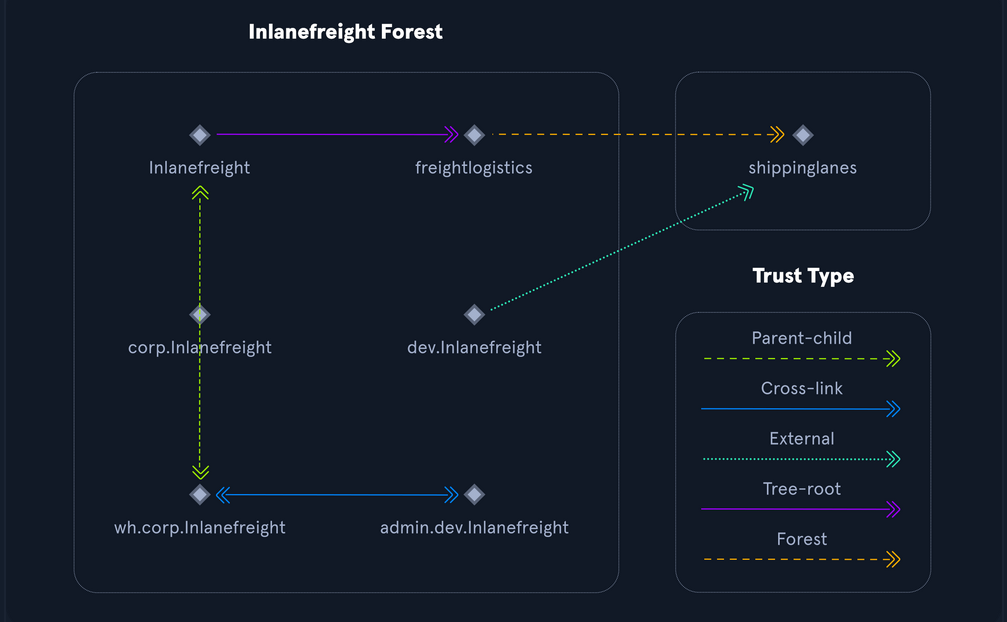
\includegraphics[width=\linewidth]{windows_knowledge/ad/images/trusts.png}
  \caption{AD trusts}
  \label{fig:ad-trusts}
\end{figure}

Trusts can be:
\begin{itemize}
\item transitive: trust is extended to objects that the child domain trusts.
\item non-transitive: only the child domain itself is trusted.
\end{itemize}


Trusts can be set up:
\begin{itemize}
    \item bidirectional: users from both trusting domains can access resources.
    \item In a one-way trust: only users in a trusted domain can access resources in a trusting domain, not vice-versa. The direction of trust is opposite to the direction of access.
\end{itemize}

Often, domain trusts are set up improperly and provide unintended  attack
paths. Also, trusts set up for ease of use may not be reviewed  later for
potential security implications. Mergers and acquisitions can  result in
bidirectional trusts with acquired companies, unknowingly  introducing risk
into the acquiring company's environment. It is not  uncommon to be able to perform an attack such as Kerberoasting against a  domain outside the principal domain and obtain a user that has  administrative access within the principal domain.

\section{Protocols}
While Windows operating systems use a variety of protocols to communicate, Active Directory specifically requires Lightweight Directory Access Protocol (LDAP), Microsoft's version of Kerberos, DNS for authentication and communication, and MSRPC.
\subsection{Kerberos}
See dedicated chapter~\ref{windows:authentication:kerberos}


\subsection{DNS}

\subsubsection{Service records}
AD maintains a database of services running on the network in the form of
\emph{service records} (\verb+SRV+). These service records allow clients in an AD environment to locate services that they need, such as a file server, printer, or Domain Controller.


Dynamic DNS is used to make changes in the DNS database automatically should a system's IP address change.

When a client joins the network, it locates the Domain Controller by sending a query to the DNS service, retrieving an SRV record from the DNS database, and transmitting the Domain Controller's hostname to the client.

\subsection{LDAP}
Active Directory supports Lightweight Directory Access Protocol (LDAP) for
directory lookups. LDAP is the language that applications use to communicate with other servers that provide directory services. 

LDAP uses port 389, and LDAP over SSL (LDAPS) communicates over port 636.

An LDAP session begins by first connecting to an LDAP server, also known as a Directory System Agent. The Domain Controller in AD actively listens for LDAP requests, such as security authentication requests.

\subsubsection{AD LDAP Authentication}

LDAP is set up to authenticate credentials against AD using a \emph{BIND}
operation to set the authentication state for an LDAP session. There are two
types of LDAP authentication :
\begin{enumerate}
    \item \emph{Simple Authentication}: This includes anonymous authentication, unauthenticated authentication, and username/password authentication. Simple authentication means that a username and password create a BIND request to authenticate to the LDAP server.

    \item \emph{SASL Authentication}: The Simple Authentication and Security Layer (SASL) framework uses other authentication services, such as Kerberos, to bind to the LDAP server and then uses this authentication service (Kerberos in this example) to authenticate to LDAP. The LDAP server uses the LDAP protocol to send an LDAP message to the authorization service, which initiates a series of challenge/response messages resulting in either successful or unsuccessful authentication. SASL can provide additional security due to the separation of authentication methods from application protocols.
\end{enumerate}

LDAP authentication messages are sent in cleartext by default so anyone can sniff out LDAP messages on the internal network. It is recommended to use TLS encryption or similar to safeguard this information in transit.

\subsection{MSRPC}
Windows systems use MSRPC to  access systems in Active Directory using four key RPC interfaces.

\begin{tabularx}{\linewidth}{|l|X|}
    \hline
Interface Name & Description \\
    \hline
lsarpc & A set of RPC calls to the Local Security Authority (LSA) system which
manages the local security policy on a computer, controls the audit policy, and
provides interactive authentication services. LSARPC is used to perform
management on domain security policies. \\
    \hline
netlogon & Netlogon is a Windows process used to authenticate users and other
services in the domain environment. It is a service that continuously runs in
the background. \\
    \hline
samr & Remote SAM (samr) provides management functionality for the domain
account database, storing information about users and groups. IT administrators
use the protocol to manage users, groups, and computers by enabling admins to
create, read, update, and delete information about security principles.
Attackers (and pentesters) can use the samr protocol to perform reconnaissance
about the internal domain using tools such as BloodHound to visually map out
the AD network and create "attack paths" to illustrate visually how
administrative access or full domain compromise could be achieved.
Organizations can protect against this type of reconnaissance by changing a
Windows registry key to only allow administrators to perform remote SAM queries
since, by default, all authenticated domain users can make these queries to
gather a considerable amount of information about the AD domain. \\
    \hline
drsuapi & drsuapi is the Microsoft API that implements the Directory
Replication Service (DRS) Remote Protocol which is used to perform
replication-related tasks across Domain Controllers in a multi-DC environment.
Attackers can utilize drsuapi to create a copy of the Active Directory domain
database (\gls{win:NTDS.DIT}) file to retrieve password hashes for all accounts in the
domain, which can then be used to perform Pass-the-Hash attacks to access more
systems or cracked offline using a tool such as Hashcat to obtain the cleartext
password to log in to systems using remote management protocols such as Remote
Desktop (RDP) and WinRM. \\
    \hline
\end{tabularx}

\subsection{NTLM}
 Active Directory uses several other authentication methods which can be used
 (and abused) by applications and services in AD.

 See dedicated chapter~\ref{windows:authentication:intlm}

\section{User and machine account}
User accounts are created on both local systems (not joined to AD) and in Active Directory to give a person or a program (such as a system service) the ability to log on to a computer and access resources based on their rights. 

When a user logs in, the system verifies their password and creates an
\gls{win:access-token}. This token describes the security content of a process or thread and includes the user's security identity and group membership. Whenever a user interacts with a process, this token is presented. 

User accounts are used to allow to log into a computer and access resources, to
run programs or services under a specific security context (i.e., running as a
highly privileged user instead of a network service account), and to manage
access to objects and their properties (network file shares, files,
applications, etc.). 

Users can be assigned to groups. These groups can also be used to control access to resources.

The ability to provision and manage user accounts is one of the core elements of Active Directory. 


Aside from standard user and admin accounts tied back to a specific user, we will often see many service accounts used to run a particular application or service in the background or perform other vital functions within the domain environment. 

As we will see later in this module, 


Because users can have so many rights assigned to them, they can also be misconfigured relatively easily and granted unintended rights. User accounts present an immense attack surface and are usually a key focus for gaining a foothold during a penetration test. Users are often the weakest link in any organization. 

An organization needs to have policies and procedures to combat issues that can arise around user accounts and must have defense in depth to mitigate the inherent risk that users bring to the domain.

\subsection{Local accounts}
\url{https://docs.microsoft.com/en-us/windows/security/identity-protection/access-control/local-accounts}

Local accounts are stored locally on a particular server or  workstation. These accounts can be assigned rights on that host either  individually or via group membership. Any rights assigned can only be  granted to that specific host and will not work across the domain. Local  user accounts are considered security principals but can only manage  access to and secure resources on a standalone host. There are several  default local user accounts that are created on a Windows system:
\begin{itemize}
    \item \emph{Administrator}: this account has the SID
        \verb+S-1-5-domain-500+  and is the first account created with a new Windows installation. It  has full control over almost every resource on the system. It cannot be  deleted or locked, but it can be disabled or renamed. Windows 10 and  Server 2016 hosts disable the built-in administrator account by default  and create another local account in the local administrator's group  during setup.

    \item \emph{Guest}: this account is disabled by default. The purpose  of this account is to allow users without an account on the computer to  log in temporarily with limited access rights. By default, it has a  blank password and is generally recommended to be left disabled because  of the security risk of allowing anonymous access to a host.

    \item \emph{SYSTEM}: (or \verb+NT AUTHORITY\SYSTEM+) is the default account installed and used by  the operating system to perform many of its internal functions. Unlike  the Root account on Linux, SYSTEM is a service account and  does not run entirely in the same context as a regular user. Many of the  processes and services running on a host are run under the SYSTEM  context. One thing to note with this account is that a profile for it  does not exist, but it will have permissions over most everything on the  host. It does not appear in User Manager and cannot be added to any  groups. A SYSTEM account is the highest permission level  one can achieve on a Windows host and, by default, is granted Full  Control permissions to all files on a Windows system.

    \item \emph{Network Service}: This is a predefined local account used  by
        the \emph{Service Control Manager} (SCM) for running Windows services. When  a service runs in the context of this particular account, it will  present credentials to remote services.

    \item \emph{Local Service}: This is another predefined local account  used by the Service Control Manager (SCM) for running Windows services.  It is configured with minimal privileges on the computer and presents  anonymous credentials to the network.
\end{itemize}

It is worth studying Microsoft's documentation on local default accounts  in-depth to gain a better understanding of how the various accounts  work together on an individual Windows system and across a domain  network. Take some time to look them over and understand the nuances  between them.

\subsection{Domain users}
Domain users differ from local users in that they are granted rights  from the domain to access resources such as file servers, printers,  intranet hosts, and other objects based on the permissions granted to  their user account or the group that account is a member of. Domain user  accounts can log in to any host in the domain, unlike local users. For  more information on the many different Active Directory account types,  check out this link. 

\url{https://docs.microsoft.com/en-us/windows/security/identity-protection/access-control/active-directory-accounts}

One account to keep in mind is the \verb+KRBTGT+  account, however. This is a
type of local account built into the AD  infrastructure. This account acts as a
service account for the Key  Distribution service providing authentication and
access for domain  resources. This account is a common target of many attackers
since  gaining control or access will enable an attacker to have unconstrained
access to the domain. It can be leveraged for privilege escalation and
persistence in a domain through attacks such as the Golden Ticket attack.
\subsubsection{User Naming Attributes}
\begin{itemize}
    \item \emph{UserPrincipalName} (UPN): This is the primary logon name for the user. By convention, the UPN uses the email address of the user.
    \item \emph{ObjectGUID}: This is a unique identifier of the user. In AD, the ObjectGUID attribute name never changes and remains unique even if the user is removed.
    \item \emph{SAMAccountName}: This is a logon name that supports the previous version of Windows clients and servers.
    \item \emph{objectSID}: The user's Security Identifier (SID). This attribute identifies a user and its group memberships during security interactions with the server.
    \item \emph{sIDHistory}: This contains previous SIDs for the user object if
        moved from another domain and is typically seen in migration scenarios
        from domain to domain. After a migration occurs, the last SID will be
        added to the sIDHistory property, and the new SID will become its
        objectSID. sIDHistory is added to the
        access-token~\ref{win:access-token}. The Mitigation is done thru
        \emph{SID Filtering}~\ref{ad:security:sid-filtering}
\end{itemize}



\subsubsection{Common user attributes}
\begin{itemize}
        \item DistinguishedName
        \item Enabled
        \item GivenName
        \item Name
        \item ObjectClass
        \item ObjectGUID
        \item Surname
\end{itemize}


\subsection{Domain-joined and Non-Domain-joined Machine}

\subsubsection{Domain joined}
Hosts joined to a domain have greater ease of information sharing  within the
enterprise and a central management point (the DC) to gather  resources,
policies, and updates from. A host joined to a domain will  acquire any
configurations or changes necessary through the domain's  Group Policy. The
benefit here is that a user in the domain can log in  and access resources from
any host joined to the domain, not just the  one they work on. This is the
typical setup you will see in enterprise  environments

\subsubsection{Non-domain joined}
Non-domain joined computers or computers in a workgroup  are not managed by
domain policy. With that in mind, sharing resources  outside your local network
is much more complicated than it would be on a  domain. This is fine for
computers meant for home use or small business  clusters on the same LAN. The
advantage of this setup is that the  individual users are in charge of any
changes they wish to make to their  host. Any user accounts on a workgroup
computer only exist on that  host, and profiles are not migrated to other hosts
within the workgroup.

It is important to note that a machine account (i\verb+NT AUTHORITY\SYSTEM+
level access) in an AD environment will have most of the same rights as  a
standard domain user account. This is important because we do not  always need
to obtain a set of valid credentials for an individual  user's account to begin
enumerating and attacking a domain. We may obtain \emph{SYSTEM level access} to
a domain-joined Windows host through a successful remote code execution
exploit or by escalating privileges on a host. This access is often  overlooked
as only useful for pillaging sensitive data (i.e., passwords,  SSH keys,
sensitive files, etc.) on a particular host. In reality,  access in the context
of the SYSTEM account will allow us  read access to much of the data within the
domain and is a great  launching point for gathering as much information about
the domain as  possible before proceeding with applicable AD-related attacks. 

\section{Active Directory Groups}
They can place similar users together and mass assign rights and access. Groups are another key target for attackers and penetration testers, as the rights that they confer on their members may not be readily apparent but may grant excessive (and even unintended) privileges that can be abused if not set up correctly. 

There are many built-in groups in Active Directoryo
The number of groups in an AD environment can snowball and become unwieldy, potentially leading to unintended access if left unchecked. 
It is essential to understand the impact of using different group types and for any organization to periodically audit which groups exist within their domain, the privileges that these groups grant their members, and check for excessive group membership beyond what is required for a user to perform their day-to-day work. 

Difference between Groups and Organizational Units (OUs): 
\begin{itemize}
        \item OU: OUs are useful for grouping users, groups, and computers:
            \begin{itemize}
                    \item to ease management and deploying Group Policy settings to specific objects in the domain. 
                    \item to delegate administrative tasks to a user, such as resetting passwords or unlocking user accounts without giving them additional admin rights that they may inherit through group membership.
            \end{itemize}
        \item Groups are primarily used to assign permissions to access resources
\end{itemize}

In simpler terms, groups are used to place users, computers, and contact objects into management units that provide ease of administration over permissions and facilitate the assignment of resources such as printers and file share access. For example, if an admin needs to assign 50 members of a department access to a new share drive, it would be time-consuming to add each user's account individually. Granting permissions this way would also make it more difficult to audit who has access to resources and difficult to clean up/revoke permissions. Instead, a sysadmin can either use an existing group or create a new group and grant that specific group permissions over the resource. From here, every user in the group will inherit the permissions based on their membership in the group. If the permissions need to be modified or revoked for one or more users, they could merely be removed from the group, leaving the other users unaffected and their permissions intact.

Groups in Active Directory have two fundamental characteristics: 
\begin{itemize}
        \item type: that defines the group's purpose;
        \item scope: shows how the group can be used within the domain or forest.
\end{itemize}


\subsection{Types of groups}
\subsubsection{Security groups}

type used to ease the assignment ofpermissions and rights to a collection of users instead. 

All users added to a security group will inherit any permissions assigned to
the group.

\subsubsection{Distribution groups}
The Distribution groups type is used by email applications to distribute messages to group members. 

This type of group cannot be used to assign permissions to resources in a domain environment.

\subsection{Scope of groups}
\begin{center}
\begin{figure}
    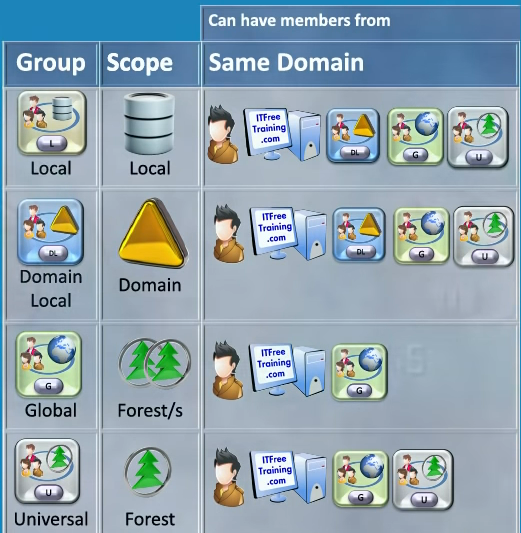
\includegraphics[width=0.5\linewidth]{windows_knowledge/ad/images/group-scopes.png}
  \caption{Group scopes overview}
  \label{fig:ad-group-scopes}
\end{figure}
\end{center}

Group scopes can be changed, but there are a few caveats:
\begin{itemize}
        \item A Global Group can only be converted to a Universal Group if it is NOT part of another Global Group.
        \item A Domain Local Group can only be converted to a Universal Group if the Domain Local Group does NOT contain any other Domain Local Groups as members.
        \item A Universal Group can be converted to a Domain Local Group without any restrictions.
        \item A Universal Group can only be converted to a Global Group if it does NOT contain any other Universal Groups as members.
\end{itemize}


\subsubsection{Domain Local}

\begin{itemize}
    \item Can only be used to manage permissions to domain resources in the domain where it was created.
    \item cannot be  used in other domains
    \item CAN contain users from OTHER domains
    \item can be nested into other local groups
    \item cannot be nested into global groups
\end{itemize}

\subsubsection{Global}
\begin{itemize}
    \item can be used to grant access to resources in another domain
    \item can only contain accounts from the domain where it was created.
    \item can be added to both other global groups and local groups
\end{itemize}

\subsubsection{Universal}
\begin{itemize}
    \item Can be used to manage resources distributed across multiple domains
    \item can be given permissions to any object within the same forest.
    \item are available to all domains within an organization
    \item can contain users from any domain.
    \item adding or removing objects from a universal group triggers forest-wide replication.
\end{itemize}

It is recommended that administrators maintain other groups (such as global groups) as members of universal groups because global group membership within universal groups is less likely to change than individual user membership in global groups.  Replication is only triggered at the individual domain level when a user is removed from a global group. 

\subsection{Built-in vs. Custom Groups}

Several
\href{https://docs.microsoft.com/en-us/windows/security/identity-protection/access-control/active-directory-security-groups}{built-in
security groups} are created with a Domain Local Group scope
when a domain is created.  These groups are used for specific administrative
purposes and are discussed more in the next section.  It is important to note
that only user accounts can be added to these built-in groups as they do not
allow for group nesting (groups within groups).

Some examples of built-in groups included Domain Admins, which is a Global security group and can only contain accounts from its own domain. 

If an organization wants to allow an account from domain B to perform administrative functions on a domain controller in domain A, the account would have to be added to the built-in Administrators group, which is a Domain Local group. 

Though Active Directory comes prepopulated with many groups, it is common for most organizations to create additional groups (both security and distribution) for their own purposes. Changes/additions to an AD environment can also trigger the creation of additional groups. For example, when Microsoft Exchange is added to a domain, it adds various different security groups to the domain, some of which are highly privileged and, if not managed properly, can be used to gain privileged access within the domain.

\subsection{Nested Group Membership}

Nested group membership is an important concept in AD. As mentioned previously, a Domain Local Group can be a member of another Domain Local Group in the same domain. Through this membership, a user may inherit privileges not assigned directly to their account or even the group they are directly a member of, but rather the group that their group is a member of. This can sometimes lead to unintended privileges granted to a user that are difficult to uncover without an in-depth assessment of the domain. Tools such as BloodHound are particularly useful in uncovering privileges that a user may inherit through one or more nestings of groups. This is a key tool for penetration testers for uncovering nuanced misconfigurations and is also extremely powerful for sysadmins and the like to gain deep insights (visually) into the security posture of their domain(s).

\subsection{Scope Strategies}
\subsubsection{AGDLP}

ADDLP stands for:
\begin{itemize}
        \item A for Accounts.
        \item G for Global Group.
        \item DL for Domain Local Group.
        \item P for Permissions.
\end{itemize}

It is a role based strategy that is designed to provide flexible resource
management using groups. It is designed for larger networks (more than 500
users). AGDLP can be used in multiple domain environments but is generally used in a single domain environment.

Since AGDLP is a role base strategy for applying permissions, as a user changes their role in an organization, it is easy to change the permissions associated to that user by making them members of the appropriate groups. Since the users are being put into groups at the role level, this means that the administrator does not require knowledge of how the permissions were applied to the resource. Lastly, by looking at the users in the groups, you can quickly determine who has access to which resources in your domain.

The basic way to use AGDLP is as follows:
\begin{itemize}
    \item Accounts go into Global Groups; 
    \item Global Groups go into Domain Local Groups;
    \item Domain Local Groups are than applied to Permissions. 
\end{itemize}

The advantage to using each group is as follows:
\begin{itemize}
    \item Global Groups allow users from the same domain to be members. This means that when using multiple domains, you can be assured that only users and computers and other Global Groups from that domain are members. This means you can force administration to be divided up between domains. If you do not use Global Groups you could never be sure if an administrator from a domain is only adding users from that domain.
    \item Domain Local Groups can only be used in the domain that the group was created in. This helps with auditing. If the group could be used in other domains, you could never be sure that the group had been applied to resources outside your domain.
\end{itemize}

AGDLP can be used in a single forest, single domain environment and also a multi domain environment. 

\url{https://www.youtube.com/watch?v=zHHzjjqVhTc}

\subsubsection{AGUDLP}

What AGUDLP standards for
\begin{itemize}
        \item A Accounts
        \item G Global Groups
        \item U Universal Groups
        \item DL Domain Local Groups
        \item P Permissions
\end{itemize}


AGUDLP can be used in multiple domain environments to provide distributed control between different domain administrators while still being able to provide access to resources at the forest level.


It allows administration to be divided up between different administrators in the forest. Administrators can have control at the forest level or control can be  separated at  the domain or resources level.

Since AGUDLP is a role base strategy, when a user changes their role, for example promoted or transferred, access can quickly and easily  be changed.

AGUDLP also allows easy auditing. By looking in the group it can quickly be determined who has access to which resources.

Why each group is used:
\begin{itemize}
    \item Global groups only contain users, computers, and other global groups
        from the same domain. If we wanted a sales
            group that had all sales users from all domains in the forest, we
            would first create a global group for the sales users in each
            domain. This allows to divide up control between
        different domains and  domain administrators in each domain to be
        responsible for keeping this group up to date. 
    \item Universal groups allow users, computers, global groups and other
        universal groups to be members. Because of this, they can have the
        global groups from all the other domains to be members of this group.
        For example, a universal group could have as members  the sales group
        from all the other domains. Universal groups are available forest wide
        and thus are replicated using the global catalog server. For this
        reason, you will want to reduce replication as much as possible in the
        forest. Replication will only occur when membership of the universal
        group has changed. Since the universal group contains global groups,
        the membership of the global groups can change without affecting the
        membership of the universal group. The only time the universal group
        would need to be replicated is when a global group is added or removed
        from the universal group.

    \item The domain local group is applied to the resources as a permission.
    Domain local groups can only be used in the domain that they were created
    in. By using domain local groups, a local domain administrator can simply
    add the domain local group to the resources and configure the appropriate
    permissions. This administrator may not have access to change the
    membership of the other groups, which means that they do not have control
    over which users go into the group. This does not affect their ability to
    use the group on local resources. This means that by using a domain local
    group, the scope of the group can be limited to use for that domain only
    and also be delegated out to other administrators. At this level, it is
    easy to add or remove the universal group to any domain local group as
    required, making changing access very quick and flexible.
\end{itemize}

\url{https://www.youtube.com/watch?v=yjPGRnxAU6M}



\section{Rights and Privileges}
\subsection{Built-in AD Groups}

AD contains many default or built-in security groups, some of which grant their
members powerful rights and privileges which can be abused to escalate
privileges within a domain and ultimately gain Domain Admin or \verb+SYSTEM+ privileges on a Domain Controller. Membership in many of these groups should be tightly managed as excessive group membership/privileges is a common flaw in many AD networks that attackers look to abuse. Some of the most common built-in groups are listed below.


\begin{xltabular}{\linewidth}{|l|X|}
    \hline
Group Name &	Description \\
    \hline
Account Operators &	can create and modify most types of accounts,
including those of users, local groups, and global groups, and members can log
in locally to domain controllers. They cannot manage the Administrator account,
administrative user accounts, or members of the Administrators, Server
Operators, Account Operators, Backup Operators, or Print Operators groups. \\
Administrators &	Members have full and unrestricted access to a computer or an
entire domain if they are in this group on a Domain Controller.\\
    \hline
Backup Operators &	can back up and restore all files on a computer,
regardless of the permissions set on the files. Backup Operators can also log
on to and shut down the computer. Members can log onto DCs locally and should
be considered Domain Admins. They can make shadow copies of the
SAM/ \gls{win:NTDS.DIT} database, which, if taken, can be used to extract credentials and other juicy
info.\\
    \hline
DnsAdmins &	have access to network DNS information. The group will only
be created if the DNS server role is or was at one time installed on a domain
controller in the domain.\\
    \hline
Domain Admins &	Members have full access to administer the domain and are
members of the local administrator's group on all domain-joined machines.\\
    \hline
Domain Computers &	Any computers created in the domain (aside from domain
controllers) are added to this group.\\
    \hline
Domain Controllers &	Contains all DCs within a domain. New DCs are added to this
group automatically.\\
    \hline
Domain Guests &	This group includes the domain's built-in Guest account.
Members of this group have a domain profile created when signing onto a
domain-joined computer as a local guest.\\
    \hline
Domain Users &	This group contains all user accounts in a domain. A new user
account created in the domain is automatically added to this group.\\
    \hline
Enterprise Admins &	Membership in this group provides complete configuration
access within the domain. The group only exists in the root domain of an AD
forest. Members in this group are granted the ability to make forest-wide
changes such as adding a child domain or creating a trust. The Administrator
account for the forest root domain is the only member of this group by
default.\\
    \hline
Event Log Readers &	Members can read event logs on local computers. The group
is only created when a host is promoted to a domain controller.\\
    \hline
Group Policy Creator Owners &	Members create, edit, or delete Group Policy
Objects in the domain.\\
    \hline
Hyper-V Administrators &	Members have complete and unrestricted access to all
the features in Hyper-V. If there are virtual DCs in the domain, any
virtualization admins, such as members of Hyper-V Administrators, should be
considered Domain Admins.\\
    \hline
IIS\_IUSRS &	This is a built-in group used by Internet Information Services
(IIS), beginning with IIS 7.0.\\
    \hline
Pre–Windows 2000 Compatible Access &	This group exists for backward
compatibility for computers running Windows NT 4.0 and earlier. Membership in
this group is often a leftover legacy configuration. It can lead to flaws where
anyone on the network can read information from AD without requiring a valid AD
username and password.\\
    \hline
Print Operators &	Members can manage, create, share, and delete printers that
are connected to domain controllers in the domain along with any printer
objects in AD. Members are allowed to log on to DCs locally and may be used to
load a malicious printer driver and escalate privileges within the domain.\\
    \hline
Protected Users &	Members of this group are provided additional protections
against credential theft and tactics such as Kerberos abuse.\\
    \hline
Read-only Domain Controllers &	Contains all Read-only domain controllers in
the domain.\\
    \hline
Remote Desktop Users &	This group is used to grant users and groups permission
to connect to a host via Remote Desktop (RDP). This group cannot be renamed,
deleted, or moved.\\
    \hline
Remote Management Users &	This group can be used to grant users remote access
to computers via Windows Remote Management (WinRM)\\
    \hline
    Schema Admins &	Members can modify the \gls{win:schema}, which is the
way all objects with AD are defined. This group only exists in the root domain
of an AD forest. The Administrator account for the forest root domain is the
only member of this group by default.\\
    \hline
Server Operators &	This group only exists on domain controllers. Members can
modify services, access SMB shares, and backup files on domain controllers. By
default, this group has no members.\\
    \hline
\end{xltabular}

\subsection{User Rights Assignment}

Depending on their current group membership, and other factors such as
privileges that administrators can assign via Group Policy (GPO), users can
have various rights assigned to their account. 

This Microsoft article on User Rights Assignment provides a detailed explanation of each of the user rights that can be set in Windows. 
\url{https://docs.microsoft.com/en-us/windows/security/threat-protection/security-policy-settings/user-rights-assignment}

some rights granted to an account can lead to unintended consequences such as privilege escalation 
or access to sensitive files. 

For example, write access over a Group Policy Object (GPO) applied to an OU
containing one or more users controled we could potentially leverage a tool
such as SharpGPOAbuse (\url{https://github.com/FSecureLABS/SharpGPOAbuse}) to assign targeted rights to a user. 
We may perform many actions in the domain to further our access with these new
rights. A few examples include :

\begin{tabularx}{\linewidth}{|l|X|}
    \hline
Privilege i&	Description \\
    \hline
SeRemoteInteractiveLogonRight &	could give our target user the
right to log onto a host via Remote Desktop (RDP). \\
    \hline
SeBackupPrivilege &	grants the ability to create system backups (copies of
    sensitive system files \verb+SAM+, \verb+SYSTEM Registry hives+ and
\gls{win:NTDS.DIT})\\ 
    \hline
SeDebugPrivilege &	allows  to debug and adjust the memory of a
process (Mimikatz to read the memory space of the LSASS process).\\
    \hline
SeImpersonatePrivilege & allows to impersonate a token of
a privileged account such as \verb+NT AUTHORITY\SYSTEM+. This could be leveraged with
a tool such as JuicyPotato, RogueWinRM, PrintSpoofer, etc., to escalate
privileges on a target system.\\
    \hline
SeLoadDriverPrivilege &	load and unload device
drivers that could potentially be used to escalate privileges or compromise a
system.\\
    \hline
SeTakeOwnershipPrivilege &	allows a process to take ownership of an
object. At its most basic level, gain access to
a file share or a file on a share that was otherwise not accessible.\\
    \hline
\end{tabularx}

\subsection{User Account Control}
\label{windows_knowledge:ad:rights_privileges:uac}

\gls{win:UAC}~\ref{windows_knowledge:fundamentals:security:uac}


\subsubsection{UserAccountControl flags attribute}
\label{windows_knowledge:ad:rights_privileges:uac:attribute}
\begin{figure}
  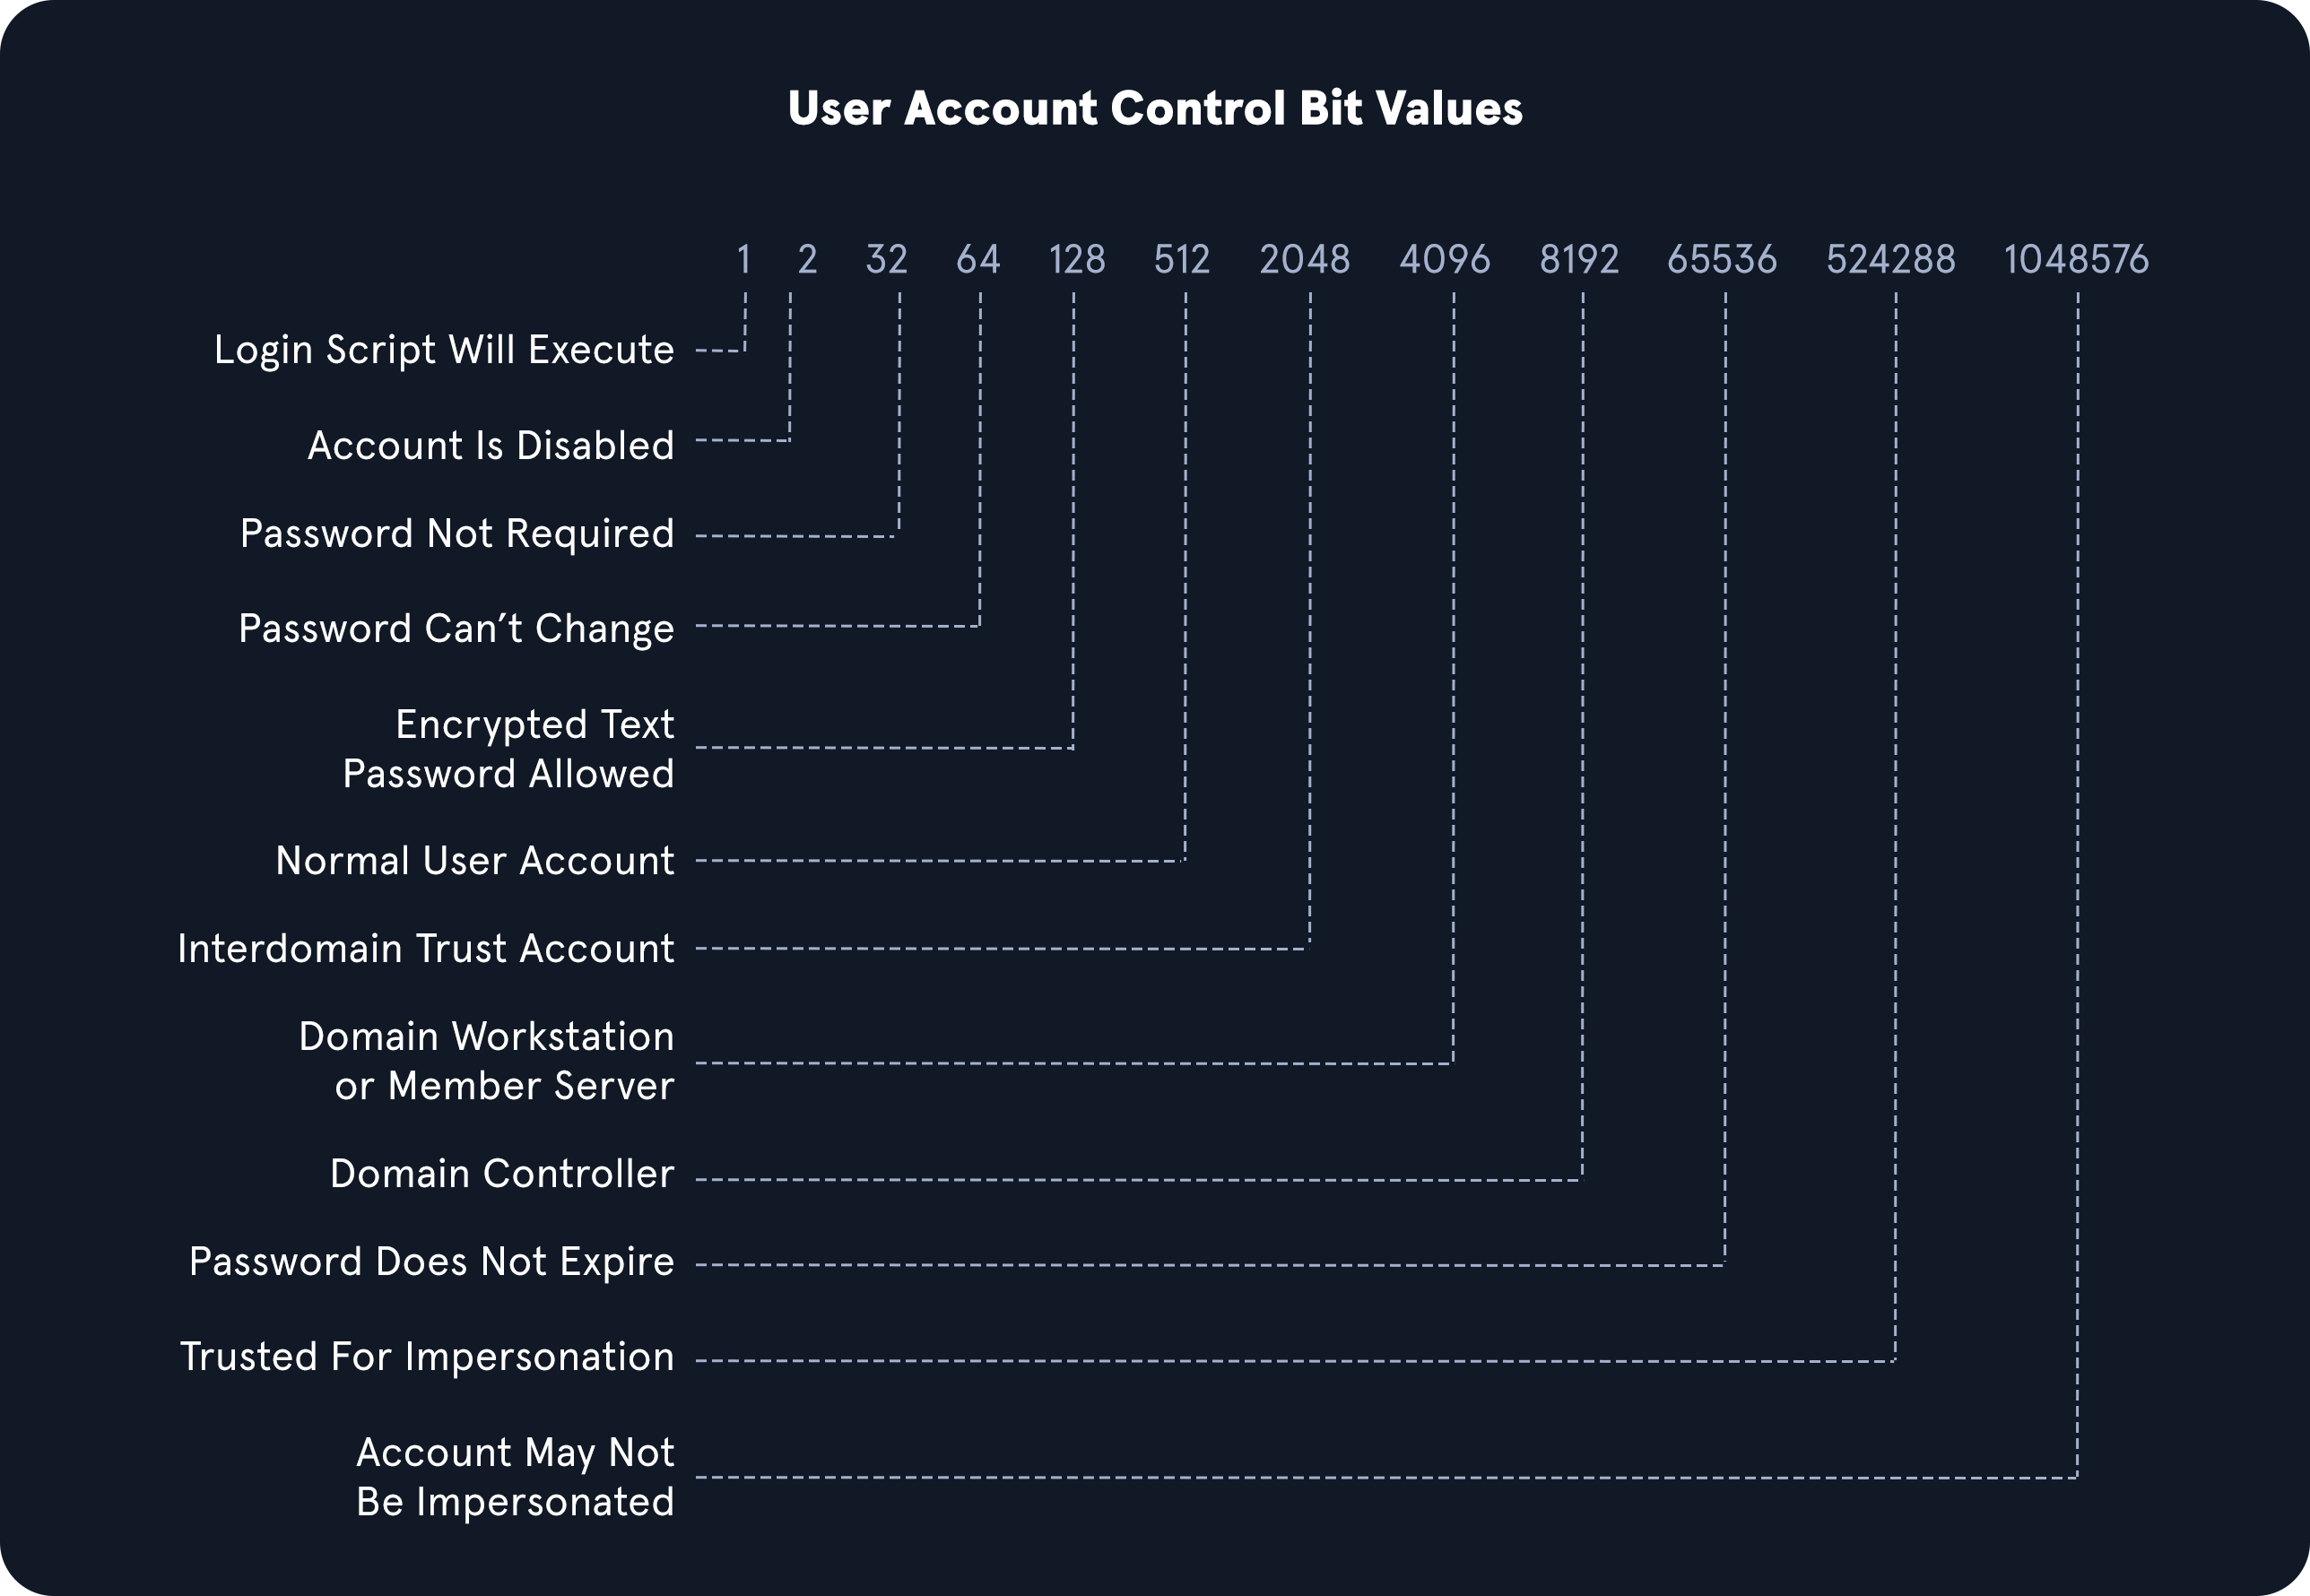
\includegraphics[width=\linewidth]{windows_knowledge/ad/images/UAC-values.png}
  \caption{Some Important UAC flag attribute values}
  \label{fig:uac-values}
\end{figure}

\subsubsection{links}

\begin{itemize}
    \item \url{https://docs.microsoft.com/en-us/windows/security/identity-protection/user-account-control/user-account-control-overview}

    \item \url{https://docs.microsoft.com/en-us/windows/security/identity-protection/user-account-control/how-user-account-control-works}
    \item
        \url{https://docs.microsoft.com/en-us/troubleshoot/windows-server/identity/useraccountcontrol-manipulate-account-properties}
\end{itemize}



\section{Security in Active Directory}

\url{https://docs.microsoft.com/en-us/security/compass/compass}

\url{https://docs.microsoft.com/en-us/windows-server/identity/ad-ds/plan/security-best-practices/best-practices-for-securing-active-directory}

Active Directory can be considered insecure by design because of  many features and functionalities are built around the premise of central management and the ability to share information quickly, at will, to a large userbase. 


A default Active Directory installation will be missing many hardening measures, settings, and tools that can be used to secure an AD implementation. 

Finding a balanced CIA Triad is hard and AD leans heavily toward Availability and Confidentiality at its core.

We can help balance the scales by utilizing Microsoft's built-in features that
can be enabled/tweaked to harden AD against common attacks. 

The list below is not exhaustive. Many other general security hardening principles must be in place within an organization to ensure a proper defense-in-depth approach (having an accurate asset inventory, vulnerability patches, configuration management, endpoint protection, security awareness training, network segmentation, etc.).

\subsection{Kerberos encryption types allowed}

It is possible to edit the encryption types used by Kerberos. This can be done
by opening Group Policy, editing the Default Domain Policy, and choosing:
Computer Configuration > Policies > Windows Settings > Security Settings >
Local Policies > Security Options, then double-clicking on Network security:
Configure encryption types allowed for Kerberos.

\subsection{Local Administrator Password Solution (LAPS)}
\label{windows_knowledge:ad:security:laps}
\href{https://www.microsoft.com/en-us/download/details.aspx?id=46899}{LAPS} is
used to randomize and rotate local administrator passwords on Windows hosts and prevent lateral movement.

\subsection{Audit Policy Settings (Logging and Monitoring)}

\subsection{Group Policy Security Settings}
\url{https://docs.microsoft.com/en-us/windows/security/threat-protection/security-policy-settings/security-policy-settings}

The following is a non-exhaustive list of the types of security policies that can be applied:
\begin{itemize}
    \item Account Policies - Manage how user accounts interact with the domain. These include the password policy, account lockout policy, and Kerberos-related settings such as the lifetime of Kerberos tickets

    \item Local Policies - These apply to a specific computer and include the security event audit policy, user rights assignments (user privileges on a host), and specific security settings such as the ability to install drivers, whether the administrator and guest accounts are enabled, renaming the guest and administrator accounts, preventing users from installing printers or using removable media, and a variety of network access and network security controls.

    \item Software Restriction Policies - Settings to control what software can be run on a host.

    \item Application Control Policies - Settings to control which applications can be run by certain users/groups. This may include blocking certain users from running all executables, Windows Installer files, scripts, etc. Administrators use AppLocker to restrict access to certain types of applications and files. It is not uncommon to see organizations block access to CMD and PowerShell (among other executables) for users that do not require them for their day-to-day job. These policies are imperfect and can often be bypassed but necessary for a defense-in-depth strategy.

    \item Advanced Audit Policy Configuration - A variety of settings that can be adjusted to audit activities such as file access or modification, account logon/logoff, policy changes, privilege usage, and more.
\end{itemize}

\subsection{Advanced Audit Policy}

\subsection{Update Management (SCCM/WSUS)}

\subsection{Protected Users Group}
\label{windows_knowledge:ad:security:protected-users-group}

The
\href{https://docs.microsoft.com/en-us/windows-server/security/credentials-protection-and-management/protected-users-security-group}{Protected
Users group} first appeared with Window Server 2012 R2. This group can be used
to restrict what members of these privileged groups can do in a domain. Adding
users to Protected Users prevents user credentials from being abused if left in
memory on a host.
The group provides the following Domain Controller and device protections:
\begin{itemize}
    \item  Group members can not be delegated with constrained or unconstrained delegation.
    \item  CredSSP will not cache plaintext credentials in memory even if Allow delegating default credentials is set within Group Policy.
    \item  Windows Digest will not cache the user's plaintext password, even if Windows Digest is enabled.
    \item  Members cannot authenticate using NTLM authentication or use DES or RC4 keys.
    \item  After acquiring a TGT, the user's long-term keys or plaintext credentials are not cached.
    \item  Members cannot renew a TGT longer than the original 4-hour TTL.
\end{itemize}


\subsection{Group Managed Service Accounts (gMSA)}
\label{windows_knowledge:ad:security:gMSA}
 
\href{https://docs.microsoft.com/en-us/windows-server/security/group-managed-service-accounts/group-managed-service-accounts-overview}{gMSA} is an account managed by the domain that offers a higher level of security than other types of service accounts for use with non-interactive applications, services, processes, and tasks that are run automatically but require credentials to run. They provide automatic password management with a 120 character password generated by the domain controller. The password is changed at a regular interval and does not need to be known by any user. It allows for credentials to be used across multiple hosts.

 \subsection{Account Separation}

Administrators must have two separate accounts. One for their day-to-day work and a second for any administrative tasks they must perform. For example, a user could log into their machine using their account to send/receive an email, create documents, etc. They should have a separate account to access a secure administrative host used to perform administrative tasks. This can help ensure that if a user's host is compromised (through a phishing attack, for example), the attacker would be limited to that host and would not obtain credentials for a highly privileged user with considerable access within the domain. It is also essential for the individual to use different passwords for each account to mitigate the risk of password reuse attacks if their non-admin account is compromised.

\subsection{Password Complexity Policies + Passphrases + 2FA}

\subsubsection{Password Policy}
\label{windows:ad:security:password_policy} 

The default password policy when a new domain is created is as follows, and
there have been plenty of organizations that never changed this policy:

\begin{tabular}{|l|c|}
    \hline
Policy &	Default Value\\
    \hline
Enforce password history &	24 days\\
    \hline
Maximum password age &	42 days\\
    \hline
Minimum password age &	1 day\\
    \hline
Minimum password length &	7\\
    \hline
Password must meet complexity requirements &	Enabled\\
    \hline
Store passwords using reversible encryption &	Disabled\\
    \hline
Account lockout duration &	Not set\\
    \hline
Account lockout threshold &	0\\
    \hline
Reset account lockout counter after &	Not set\\
    \hline
\end{tabular}

\subsection{Limiting Domain Admin Account Usage}
All-powerful Domain Admin accounts should only be used to log in to Domain Controllers, not personal workstations, jump hosts, web servers, etc. This can significantly reduce the impact of an attack and cut down potential attack paths should a host be compromised. This would ensure that Domain Admin account passwords are not left in memory on hosts throughout the environment.

\subsection{Periodically Auditing and Removing Stale Users and Objects}

It is important for an organization to periodically audit Active Directory and remove or disable any unused accounts. For example, there may be a privileged service account that was created eight years ago with a very weak password that was never changed, and the account is no longer in use. Even if the password policy had since been changed to be more resistant to attacks such as password spraying, an account such as this may be a quick and easy foothold or method for lateral movement or privilege escalation within the domain.

\subsection{Auditing Permissions and Access}

Organizations should also periodically perform access control audits to ensure that users only have the level of access required for their day-to-day work. It is important to audit local admin rights, the number of Domain Admins (do we really need 30 of them?), and Enterprise Admins to limit the attack surface, file share access, user rights (i.e., membership in certain privileged security groups), and more.

\subsection{Audit Policies and Logging}

Visibility into the domain is a must. An organization can achieve this through robust logging and then using rules to detect anomalous activity (such as many failed login attempts that could be indicative of a password spraying attack) or indicators that a Kerberoasting attack is being attempted. These can also be used to detect Active Directory enumeration. It is worth familiarizing ourselves with Microsoft's Audit Policy Recommendations to help detect compromise.

\subsection{Using Restricted Groups}

Restricted Groups allow for administrators to configure group membership via Group Policy. They can be used for a number of reasons, such as controlling membership in the local administrator's group on all hosts in the domain by restricting it to just the local Administrator account and Domain Admins and controlling membership in the highly privileged Enterprise Admins and Schema Admins groups and other key administrative groups.

\subsection{Limiting Server Roles}

It is important not to install additional roles on sensitive hosts, such as installing the Internet Information Server (IIS) role on a Domain Controller. This would increase the attack surface of the Domain Controller, and this type of role should be installed on a separate standalone web server. Some other examples would be not hosting web applications on an Exchange mail server and separating web servers and database servers out to different hosts. This type of role separation can help to reduce the impact of a successful attack.

\subsection{Limiting Local Admin and RDP Rights}

Organizations should tightly control which users have local admin rights on which computers. As stated above, this can be achieved using Restricted Groups. I have seen too many organizations with the entire Domain Users group with local admin rights on one or more hosts. This would allow an attacker that compromises ANY account (even a very low privileged one) to access that host as a local admin and potentially obtain sensitive data or steal high privileged domain account credentials from memory if another user is logged in. The same goes for Remote Desktop (RDP) rights. If many users can RDP to one or many machines, this increases the risk of sensitive data exposure or potential privilege escalation attacks, leading to further compromise.

\subsection{SID filtering}
\label{ad:security:sid-filtering}

\href{https://www.serverbrain.org/active-directory-2008/sid-history-and-sid-filtering.html}{SID
Filtering} is a protection put in place to filter out authentication requests
from a domain in another forest across a trust. 


\section{Group Policy}
\label{windows:ad:gpo}
While Group Policy is an excellent tool for managing the security of a domain,
it can also be abused. Gaining rights over a Group Policy Object could lead to
lateral movement, privilege escalation, and even full domain compromise.

They can also be used as a way for an attacker to maintain persistence within a network. 

\subsection{GPO}
\index{Active Directory!Group Policy Object}
\url{https://docs.microsoft.com/en-us/previous-versions/windows/desktop/policy/group-policy-objects}

A \gls{win:GPO} is a virtual collection of policy settings that can
be applied to user(s) or computer(s). 

Every \gls{win:GPO} has a unique name and is assigned a unique \gls{win:GUID}. 

They can be linked to a specific \gls{win:OU}, \gls{win:domain}, or \gls{win:site}. 

\subsection{Order of Precedence}
GPOs are processed from the top down when viewing them from a domain organizational standpoint. 

A GPO linked to an OU at the highest level in an Active Directory network (at the domain level, for example) would be processed first, followed by those linked to a child OU, etc. 

One more thing to keep track of with precedence is that a setting configured in Computer policy will always have a higher priority of the same setting applied to a user.

\begin{tabularx}{\linewidth}{|l|X|}
    \hline
Level &	Description \\
    \hline
Local Group Policy &	The policies are defined directly to the host locally
outside the domain. Any setting here will be overwritten if a similar setting
is defined at a higher level. \\
    \hline
Site Policy  &	Any policies specific to the Enterprise Site that the host
resides in. Access Control policies are a great example of this. This is also a
great way to perform actions like printer and share mapping for users in
specific sites. \\
    \hline
Domain-wide Policy & Any settings you wish to have applied across the domain as
a whole. For example, setting the password policy complexity level, configuring
a Desktop background for all users, and setting a Notice of Use and Consent to
Monitor banner at the login screen. \\
    \hline
Organizational Unit (OU) & These settings would affect users and computers who
belong to specific OUs. You would want to place any unique settings here that
are role-specific. For example, the mapping of a particular share drive that
can only be accessed by HR, access to specific resources like printers, or the
ability for IT admins to utilize PowerShell and command-prompt. \\
    \hline
nested OU Policies &	Settings at this level would
reflect special permissions for objects within nested OUs. For example,
providing Security Analysts a specific set of Applocker policy settings that
differ from the standard IT Applocker settings. \\
    \hline
\end{tabularx}

We can manage Group Policy from the Group Policy Management Console or using the PowerShell GroupPolicy module via command line. 

The Default Domain Policy is the default GPO that is automatically created and linked to the domain. 

It has the highest precedence of all GPOs and is applied by default to all users and computers. 

Generally, it is best practice to use this default GPO to manage default settings that will apply domain-wide. 

The Default Domain Controllers policy is also created automatically with a domain and sets baseline security and auditing settings for all domain controllers in a given domain. It can be customized as needed, like any GPO.

\subsubsection{Enforced GPO Policy Precedence}

It is possible to specify the \verb+Enforced+ option to enforce settings in a specific GPO. 

If this option is set, policy settings in GPOs linked to lower OUs CANNOT override the settings. 

If a GPO is set at the domain level with the Enforced option selected, the settings contained in that GPO will be applied to all OUs in the domain and cannot be overridden by lower-level OU policies. 

\subsubsection{Block inheritance}
It is also possible to set the \verb+Block inheritance+ option on an OU. If this is specified for a particular OU, then policies higher up (such as at the domain level) will NOT be applied to this OU. If both options are set, the No Override option has precedence over the Block inheritance option. 

\subsection{Group Policy Refresh Frequency}

We can modify the refresh interval via Group Policy by clicking on Computer Configuration --> Policies --> Administrative Templates --> System --> Group Policy and selecting Set Group Policy refresh interval for computers

\subsection{Security Considerations of GPOs}

As mentioned earlier, GPOs can be used to carry out attacks. These attacks may include adding additional rights to a user account that we control, adding a local administrator to a host, or creating an immediate scheduled task to run a malicious command such as modifying group membership, adding a new admin account, establishing a reverse shell connection, or even installing targeted malware throughout a domain. These attacks typically happen when a user has the rights required to modify a GPO that applies to an OU that contains either a user account that we control or a computer.





\section{links}
\begin{itemize}
\item \url{https://docs.microsoft.com/en-us/windows/win32/adschema/attributes-all}
\item \url{}
\item \url{}
\item \url{}
\end{itemize}
